\documentclass[12pt]{amsart}
\usepackage{url,amsmath,amsthm,enumitem,amsfonts,tikz,verbatim,amssymb, wasysym, clrscode3e, booktabs, soul}
% \usepackage[doublespacing]{setspace}
\usepackage[makeroom]{cancel}
\usetikzlibrary{arrows}

\title{ University of Massachusetts Lowell \protect\\
	DEPARTMENT OF MATHEMATICAL SCIENCES \protect\\
MATH 4750 \protect\\
Updated proposal for Senior Seminar}
\author{Joel Savitz \\ Summer  2020 \\ SID: 01739537}

\newcommand{\reals}{\mathbb{R}}

\begin{document}

\maketitle

\section{Background}

Scientists express physical laws of
the universe in the language of differential equations.
The reason for this is not immediately obvious,
though my personal work with differential equations
has provided me with an induition as to why.
Fortunately for me,
Siddiqi describes three necessary properties
of a physical law that are satisfied by a differential equation \cite{whydiffeq}:


\begin{itemize}
	\item ``The mathematical relation must be sufficiently general"
	\item ``It must define connections between neighboring points"
	\item ``It must imply the continuity of change"
\end{itemize}

Differential equations satisfy all three of these properties
since they are general enough that
changes to the initial values of a system
do not violate the constraints defined by a general solution
and the relationship between a function and one or more of its derivates
defines the connection between points in the domain of the function
and implies that change in the system is continuous
due to the nature of calculus.

\section{Proposal: Verification of physical laws}

For my senior seminar project,
I propose a study of
the differential equations describing several physical laws
by way of verification
using hardware sensors
for the Raspbery Pi computer.

Specifically, I plan to verify Newton's law of cooling
using a sensor such the DS18D20,
a waterproof temperature sensor compatible with the Raspberry Pi.
These sensors are relatively innexpensive,
with a 5 pack selling for $\$12.98$ on Amazon \cite{Amazon}.

Newton's law of cooling states that
``the rate of heat loss of a body is
directly proportional to the difference
in the temperatures between the body and
its surroundings" \cite{wiki}.

If we let $T: \reals \to \reals$ be the temperature
of some body at a time $t$
and let $A$ be the ambient temperature
surrounding the body,
we have that equation \ref{eq1}
describes Newton's law of cooling.

\begin{align} \label{eq1}
	\frac{dT}{dt} = -k(T - A) \textrm{ for some $k \in \reals$}
\end{align}

I will verify this law by experiementation.

\section{Timeline}

I propose a timeline for this project in figure \ref{timeline}
in the same manner as I propose the timeline for
my larger honors project to which this
mathematical project is related \cite{rpi_plan}.

\subsection{Essential goals}

\begin{enumerate}
	\item[A1.] Verification of Newton's law of colling
	\item[A2.] Submission of archivable document describing this work
\end{enumerate}


\begin{figure}

  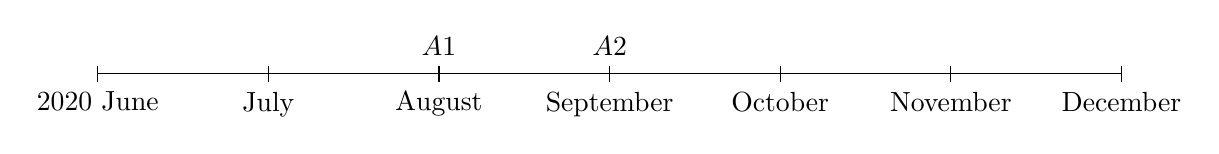
\begin{tikzpicture}
    % draw horizontal line   
    \draw (0,0) -- (13,0);

    % draw vertical lines
    \foreach \x in {0,2.166, 4.333, 6.5, 8.666, 10.833, 13}
      \draw (\x cm,3pt) -- (\x cm,-3pt);

    % draw nodes
      \draw (0,0) node[below=3pt] {$ \textrm{2020 June}$} node[above=3pt] {$  $};
      \draw (2.166,0) node[below=3pt] {$ \textrm{July} $} node[above=3pt] {$  $};
      \draw (4.333,0) node[below=3pt] {$ \textrm{August} $} node[above=3pt] {$ A1 $};
      \draw (6.500,0) node[below=3pt] {$ \textrm{September} $} node[above=3pt] {$ A2 $};
      \draw (8.666,0) node[below=3pt] {$ \textrm{October} $} node[above=3pt] {$  $};
      \draw (10.833,0) node[below=3pt] {$ \textrm{November} $} node[above=3pt] {$ $};
    \draw (13,0) node[below=3pt] {$ \textrm{December} $} node[above=3pt] {$ $};
  \end{tikzpicture}

  \centering
  \caption{Proposed timeline for this project}
  \label{timeline}

\end{figure}

\bibliographystyle{plain}
\bibliography{timeline}

\end{document}
